% Copyright (C) 2007 Technical University of Liberec.  All rights reserved.
%
% Please make a following reference to Flow123d on your project site if you use the program for any purpose,
% especially for academic research:
% Flow123d, Research Centre: Advanced Remedial Technologies, Technical University of Liberec, Czech Republic
%
% This program is free software; you can redistribute it and/or modify it under the terms
% of the GNU General Public License version 3 as published by the Free Software Foundation.
%
% This program is distributed in the hope that it will be useful, but WITHOUT ANY WARRANTY;
% without even the implied warranty of MERCHANTABILITY or FITNESS FOR A PARTICULAR PURPOSE.
% See the GNU General Public License for more details.
%
% You should have received a copy of the GNU General Public License along with this program; if not,
% write to the Free Software Foundation, Inc., 59 Temple Place - Suite 330, Boston, MA 021110-1307, USA.
%
%%%%%%%%%%%%%%%%%%%%%%%%%%%%%%%%%%%%%%%%%%%%%%%%%%%%%%%%%%%%%%%%%%
%
% use PDFLatex to compile this
%

\documentclass[a4paper]{article}

% our own flow_doc.sty
%\usepackage{flow_doc}

%\usepackage{rotating}
%\usepackage{pdflscape}

\usepackage{amssymb, amsmath, amsthm}
\newtheorem{theorem}{Theorem}


\usepackage{array}
\usepackage{longtable}
\usepackage[usenames,dvipsnames]{color}   %colors
%\usepackage{colortbl}   %colorful tables
\usepackage{tabularx}
\usepackage{graphicx} %[dvips]
% it is note used \usepackage{cooltooltips}

%these two can be found in caption package
%\usepackage{caption}
%\usepackage{subcaption}

\usepackage[numbers]{natbib}

%\usepackage{fancyvrb}   % extended verbatim environments (for examples of IO files)

%\usepackage{multicol}
\usepackage{etoolbox}


%%%%%%%%%%%%%%%%%%%%%%%%%%%%%%%%%%%%%%%%%%%%%%%%%%%%%%%%%%%%%%%%%%%%%%%%%%%%
% macro for units 
\def\UNIT#1#2{\ifstrempty{#2}{}{%
\ifstrequal{#2}{1}{\mathrm{#1}}{\mathrm{#1}^{#2}}%
}}
\def\units#1#2#3{\ifstrempty{#1#2#3}{$[-]$}{$[ \UNIT{kg}{#1}\UNIT{m}{#2}\UNIT{s}{#3} ]$}}       %with brackets
\def\unitss#1#2#3{\ifstrempty{#1#2#3}{$-$}{$ \UNIT{kg}{#1}\UNIT{m}{#2}\UNIT{s}{#3} $}}  %without brackets


\newcommand{\vari}[1]{{\it #1}}
\newcommand{\ditem}[2]{\item[\vari{#1} {\tt #2}]}
\newenvironment{fileformat}{\tt\begin{flushleft}}{\end{flushleft}}

%%%%%%%%%%%%%%%%%%%% specific math macros
\def\prtl{\partial}
\def\vc#1{\mathbf{\boldsymbol{#1}}}     % vector
\def\tn#1{{\mathbb{#1}}}    % tensor
\def\abs#1{\lvert#1\rvert}
\def\Abs#1{\bigl\lvert#1\bigr\rvert}
\def\div{\operatorname{div}}
\def\ep{\varepsilon}
\def\ff{\vc f}
\def\Lapl{\Delta}
\def\grad{\nabla}
\def\Real{{\mathbf R}}
\def\d {\,{\rm d}}
\def\Natural{\mathbf N}
\def\nn{\vc n}
\def\norm#1{\|#1\|}
\def\ol{\overline}
\def\tr{\operatorname{tr}}
\def\ul{\underline}
\def\uu{\vc u}
\def\vv{\vc v}
\def\yy{{\vc y}}

\newcommand{\note}[2]{{\color{blue} \textbf{ #1:} \textit{#2}}}
%% ini_table members
%%%%%%%%%%%%%%%%%%%% specific math macros


%%%%%%%%%%%%%%%%%%%%%%%%%%%%%%%%%%%%%%%%%%%%%%%%%%%%%%%%%%%%%%%%%%%%%%%%%%%%%%%%%%%%%%%%%%%%% BEGIN DOCUMENT
%% set specific page layout
%\addtolength{\textwidth}{2cm}
%\addtolength{\hoffset}{-1.5cm}
%\addtolength{\textheight}{4cm}
%\addtolength{\voffset}{-2.5cm}
\begin{document}

\title{Continuum-fracture model for Biot poroelasticity}
\maketitle

\section{Introduction}


\begin{figure}[h]
\centering
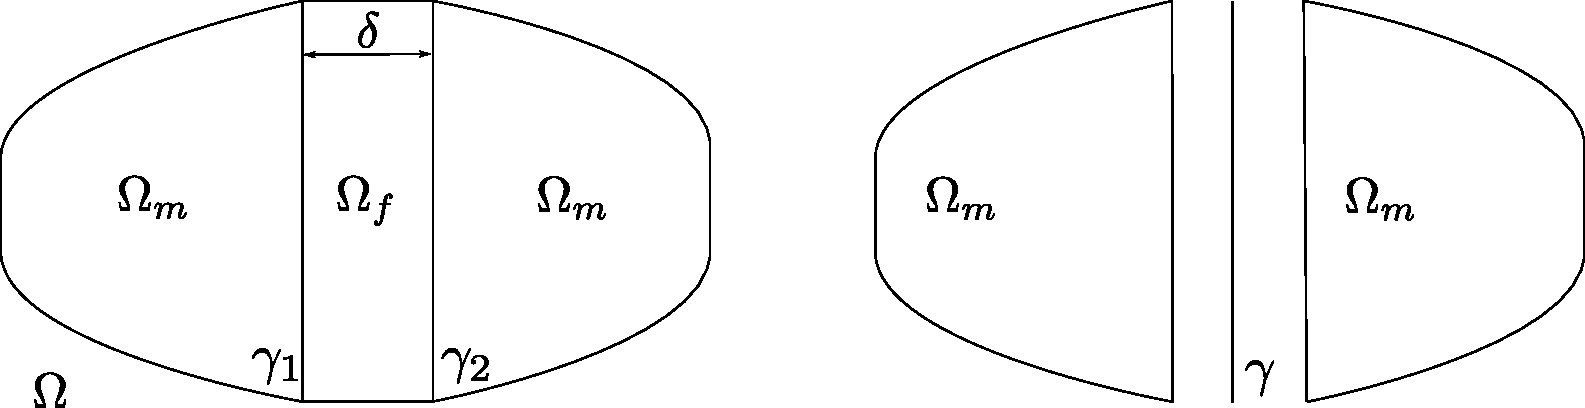
\includegraphics[width=12cm]{figures/full_model_domain}
\label{fig:omegas}
\caption{The domain of the full model (left) and the reduced geometry (right).}
\end{figure}

We consider a bounded domain $\Omega \subset \Real^d$, $d=2,3$ with a Lipschitz boundary, see Figure \ref{fig:omegas} left). The domain $\Omega$ contains 
a fracture $\Omega_f:=\Omega\cap \big((-\delta/2,\delta/2)\times\Real^{d-1}\big)$ 
with the aperture $\delta>0$ surrounded by the matrix domain $\Omega_m:=\Omega\setminus\overline\Omega_f$. 
The left and right part of $\Omega_m$ will be denoted by $\Omega_{m1}$ and $\Omega_{m2}$, respectively.
% \note{JB}{$\Omega_m$ is not simply connected, thus not domain; are there some important consequences?}
The fracture interacts with the matrix domain on the interfaces 
$\gamma_1:=\Omega\cap\big( \{-\delta/2\}\times \Real^{d-1}\big)$ and 
$\gamma_2:=\Omega\cap\big( \{ \delta/2\}\times \Real^{d-1}\big)$. Normal vectors of these interfaces are denoted $\vc n_i$, $i=1,2$ with orientation out of the domain $\Omega_m$.
Further, we introduce reduced geometry (see Figure \ref{fig:omegas})
where the fracture domain is represented by the interface $\gamma:=\Omega\cap\big(\{0\}\times\Real^{d-1}\big)$ in its center. 

We shall derive a model of poroelasticity on the reduced geometry.
The starting point is the Biot system:
\begin{subequations}
\label{eq:biot}
\begin{align}
    \label{eq:lin_el}
    -\div \vc\sigma[\uu,p] &= \ff &&\mbox{ in }\Omega, \\
    \prtl_t\left(\frac{p}{M} + \div(\alpha\uu)\right)-\div(\tn K\nabla p) &= g &&\mbox{ in }\Omega,
\end{align}
\end{subequations}
where
\[ \vc \sigma[\uu,p] = \tn C\ep[\uu]-\alpha p\tn I,~\ep[\uu]=\frac12(\nabla\uu+\nabla^\top\uu). \]





\section{Continuum-fracture model for elasticity}
\label{sc:ad_on_fractures}

In this section, we shall integrate the equation \eqref{eq:lin_el} across the fracture and obtain its approximation on the surface $\gamma$ running through the middle of the fracture.

% For the sake of simplicity, we will not write subscript $f$ for quantities on the fracture. 
By $x$, $\vc y$, we denote the normal and the tangential coordinate of a point in $\Omega_f$.
Accordingly, we denote the crosswind and the tangential part of a vector $\vv$ and a matrix $\tn A$:
\[ v_x := \vv\cdot\nn_1, \quad \vv_\yy := \vv-v_x\nn_1, \]
\[ \vc A_x := \tn A\nn_1, \quad \tn A_\yy := \tn A-\vc A_x\otimes\nn_1 = \tn A(\tn I-\nn_1\otimes\nn_1). \]
The crosswind, the tangential derivative and the tangential divergence, respectively, is defined by
\[ \prtl_x\vv := (\nabla\vv)_x,\quad \nabla_\yy\vv := (\nabla\vv)_\yy,\quad \div_\yy\vv:=\div(\vv_\yy),\quad \div_\yy\tn A:=\div\tn A_\yy. \]
% For vector-valued functions we define
% \[ \nabla_\yy\vv:=\begin{pmatrix}
% 0 & \prtl_{y_1}v_x  & ... & \prtl_{y_{d-1}} v_x\\
% 0 & \prtl_{y_1}v_{y_1}  & ... & \prtl_{y_{d-1}} v_{y_1}\\
% &&...\\
% 0 & \prtl_{y_1}v_{y_{d-1}}  & ... & \prtl_{y_{d-1}} v_{y_{d-1}}
% \end{pmatrix} \]
% and $\div_\yy\vv:=\tr\nabla_\yy\vv = \sum_{i=1}^{d-1}\prtl_{y_i} v_{y_i}$.
% For a matrix-valued function
% \[ \tn A=\begin{pmatrix}
% a_{xx} & a_{xy_1} & ... & a_{xy_{d-1}}\\
% a_{y_1x} & a_{y_1y_1} & ... & a_{y_1y_{d-1}}\\
% &&...\\
% a_{y_{d-1}x} & a_{y_{d-1}y_1} & ... & a_{y_{d-1}y_{d-1}}
% \end{pmatrix} \]
% we define
% \[ \div_\yy\tn A = \begin{pmatrix}
% \prtl_{y_1}a_{xy_1}+...+\prtl_{y_{d-1}}a_{xy_{d-1}}\\
% \prtl_{y_1}a_{y_1y_1}+...+\prtl_{y_{d-1}}a_{y_1y_{d-1}}\\
% ...\\
% \prtl_{y_1}a_{y_{d-1}y_1}+...+\prtl_{y_{d-1}}a_{y_{d-1}y_{d-1}}
% \end{pmatrix}. \]
The symbol
\[ \overline w:=\frac1\delta\int_{-\delta/2}^{\delta/2} w(x,\cdot)\,dx \]
will denote the integral mean of a function $w$ across the fracture opening.


We assume that $\tn C(x, \vc y)=\tn C(\vc y)$ is constant in the normal direction of $\Omega_f$.
Further we assume the usual symmetries of $\tn C$, i.e.
\[ \forall i,j,k,l=1,\ldots,d:~ c_{ijkl}=c_{jikl}=c_{ijlk}=c_{klij}. \]
% In order to make the procedure mathematically correct, we have to assume that the functions
% $\prtl_x w$, $\prtl_x \grad_{\vc y} u$, $\prtl_x \vc b_{\vc y}$ are continuous and bounded on $\Omega_f$, moreover
We decompose the term on the left hand side of \eqref{eq:lin_el} as follows:
\begin{equation}
\label{eq:decomp_div_sigma}
\div\vc\sigma[\uu,p] = \prtl_x(\vc\sigma[\uu,p]\nn_1) + \div_y(\tn C\nabla_y\uu + \tn C(\prtl_x\uu\otimes\nn_1) - \alpha p\tn I)
\end{equation}
and integrate over the fracture opening $[-\delta/2,\delta/2]$:
\begin{multline}
    \label{eq:integrate_div_sigma}
   \int_{-\delta/2}^{\delta/2}\div\vc\sigma[\uu,p]~dx
   = -\vc \sigma[\uu_2,p_2]\nn_2 - \vc \sigma[\uu_1,p_1]\nn_1\\
   + \div_\yy(\delta\tn C\nabla_\yy\uu_f) + \div_\yy(\sum_{i=1}^2\tn C(\uu_f-\uu_i)\otimes\nn_i)
   - \div_\yy(\delta\alpha p_f\tn I),
\end{multline}
where $\uu_f:=\overline\uu$, $p_f:=\overline p$, $\uu_i:=\uu_{|\Omega_{mi}}$ and $p_i:=p_{|\Omega_{mi}}$, $i=1,2$.
Further we approximate:
\begin{equation}
\label{eq:approx_sigma_flux}
\vc\sigma[\uu_2,p_2]\nn_2 = \frac2\delta\int_0^{\delta/2}\vc\sigma[\uu,p]\nn_2~dx + O(\delta^2),
\end{equation}
where
\begin{multline}
\frac2\delta\int_0^{\delta/2}\vc\sigma[\uu,p]\nn_2 = \frac2\delta\int_0^{\delta/2}\left(\tn C(\nabla_\yy\uu)+\tn C(\prtl_x\uu\otimes\nn_1)-\alpha p\tn I\right)\nn_2~dx\\
\approx \tn C(\nabla_\yy\uu_f)\nn_2 - \frac2\delta\tn C((\uu_2-\uu_f)\otimes\nn_2)\nn_2 - \frac{\alpha_2p_2+\alpha^f p_f}2\nn_2 =: \vc q_2.
\end{multline}
Similarly we get
\begin{equation}
\label{eq:integrate_sigma_flux_1}
\vc\sigma[\uu_1,p_1]\nn_1 \approx \tn C(\nabla_\yy\uu_f)\nn_1 - \frac2\delta\tn C((\uu_1-\uu_f)\otimes\nn_1)\nn_1 - \frac{\alpha_1p_1+\alpha^f p_f}2\nn_1 =: \vc q_1.
\end{equation}
Consequently, we obtain from \eqref{eq:lin_el} and \eqref{eq:decomp_div_sigma}--\eqref{eq:integrate_sigma_flux_1} the continuum-fracture system for linear elasticity:
\[ \begin{aligned}
-\div_\yy(\delta\vc\sigma_\yy[\uu_f,p_f]) + \sum_{i=1}^2\left(\div_\yy(\tn C(\uu_i-\uu_f)\otimes\nn_i) - \vc q_i\right) &= \delta\overline\ff &&\mbox{ in }\gamma, \\
-\div\vc\sigma[\uu_i,p_i] &= \ff &&\mbox{ in }\Omega_{mi}, \\
\vc\sigma[\uu_i,p_i]\nn_i &= \vc q_i &&\mbox{ on }\gamma_i,~i=1,2. \end{aligned} \]








\bibliographystyle{abbrvnat}
\bibliography{flow123d_doc.bib}
%%%%%%%%%%%%%%%%%%%%%%%%%%%%%%%%%%%%%%%%%%%%%%%%%%%%%%%%%%%%%%%%%%%%%%%%%%%%%%%%%%%%%%%%%%%%%%%%%%%%%%%%%%%%%%%%%


\end{document}


